\documentclass[12pt,a4paper]{article}
\usepackage[margin=0.5in]{geometry} % custom margins
\usepackage{graphicx}
\graphicspath{ {./Images/} }
\usepackage{array,mathtools}
\usepackage{listings}

% When writing indented paragraphs:
% \usepackage{indentfirst}

% To supress page numbers:
% \usepackage{nopageno}

\begin{document}
\begin{center}
    
\includegraphics[width=\textwidth]{./Images/Header.jpeg}
    \vfill
    \textbf{\Large{Report for Experiment \#6\\
    }}
    \vfill
    Trevor Smith\\
    \today
    \vfill
\end{center}

\newpage


\section*{Prelab:}
\subsection*{Lab 6}

First we'll just define each of these variables to avoid losing our minds. \\

\begin{itemize}
	\item OPcode - input instruction
	\item RegDst - toggles wether to use rt (0) or rd (1) for RegWrite location.
		for R-type, this is 1 - for I-type, it's 0.
	\item RegWrite - 1 if a value will be stored in a register, 0 otherwise. Not sure of any
		examples where this would be 0 at present moment.
	\item ALUSrc1 - Toggles between input soureces ReadData1 and \$0 into the ALU - 0
		for ReadData1 and 1 for \$0 (obviously).
	\item ALUSrc2 - Toggles between input sources ReadData2 (0) and an immediate (1) to
		the ALU. Will generally be 1 for immediate instructions.
	\item ALUOp - determines the ALU operation. These are given by the instruction set
		reference.
	\item MemWrite - 1 if storing memory
	\item MemToReg - 1 if memory is to be stored in the regfile, 0 if the ALU result
		is to be stored in the reg file.
\end{itemize}

\begin{centering}
\begin{tabular}{||c||c|c|c|c|c|c|c|c|c|}
	\hline
	\hline
	Alias & OPcode & RegDst & RegWrite & ALUSrc1 & ALUSrc2 & ALUOp[2:0] & MemWrite & MemToReg \\ \hline
	\hline
	lw    & 0000   & 1'b0   & 1'b1     & 1'b0    & 1'b1    & 3'b000     & 1'b0     & 1'b1     \\ \hline
	sw    & 0001   & 1'bx   & 1'b0     & 1'b0    & 1'b1    & 3'b000     & 1'b1     & 1'bx     \\ \hline
	add   & 0010   & 1'b1   & 1'b1     & 1'b0    & 1'b0    & 3'b000     & 1'b0     & 1'b0     \\ \hline
	addi  & 0011   & 1'b0   & 1'b1     & 1'b0    & 1'b1    & 3'b000     & 1'b0     & 1'b0     \\ \hline
	inv   & 0100   & 1'b1   & 1'b1     & 1'b1    & 1'b0    & 3'b001     & 1'b0     & 1'b0     \\ \hline
	and   & 0101   & 1'b1   & 1'b1     & 1'b0    & 1'b0    & 3'b010     & 1'b0     & 1'b0     \\ \hline
	andi  & 0110   & 1'b0   & 1'b1     & 1'b0    & 1'b1    & 3'b010     & 1'b0     & 1'b0     \\ \hline
	or    & 0111   & 1'b1   & 1'b1     & 1'b0    & 1'b0    & 3'b011     & 1'b0     & 1'b0     \\ \hline
	ori   & 1000   & 1'b0   & 1'b1     & 1'b0    & 1'b1    & 3'b011     & 1'b0     & 1'b0     \\ \hline
	sra   & 1001   & 1'b0   & 1'b1     & 1'b0    & 1'bx    & 3'b100     & 1'b0     & 1'b0     \\ \hline
	sll   & 1010   & 1'b0   & 1'b1     & 1'b0    & 1'b1    & 3'b101     & 1'b0     & 1'b0     \\ \hline
	beq   & 1011   & 1'b0   & 1'b0     & 1'b0    & 1'b0    & 3'b110     & 1'b0     & 1'bx     \\ \hline
	bne   & 1100   & 1'b0   & 1'b0     & 1'b0    & 1'b0    & 3'b111     & 1'b0     & 1'bx     \\ \hline
	clr   & 1101   & 1'b0   & 1'b1     & 1'b1    & 1'b0    & 3'b010     & 1'b0     & 1'b0     \\ \hline
\end{tabular}
\end{centering}

beq has unclear implementation in the current diagram - e.g. are we using RegWrite=1 to write to a \$ra
reg? \\

\begin{lstlisting}
inv $1, $1
sll $1, $1, 0x03
sw $1, 0xFF($3)
lw $2, 0xFF($3)
ori $2, $2, 0xF0
\end{lstlisting}

The machine code for the above is:\\
0100000101000000 \\
1010010100000011 \\
0001110111111111 \\
0000111011111111 \\
1000101011110000

\subsection*{Lab 7}
\begin{lstlisting}
addi $0, $2, 0x10
addi $1, $2, 0x0F
sw $0, 0($4)
sw $1, 0($5)
lw $0, 0($4)
sw $1, 0($5)
add $0, $0, $1
sw $0, 0($11)
lw $0, 0($5)
inv $0, $0
addi $0, $0, 1
sw $0, 0($12)
lw $0, 0($4)
lw $1, 0($12)
add $0, $0, $1
sw $0, 0($13)
\end{lstlisting}

The generated machine code is: \\
3810,390f,1000,1500,0000,1500,2100,1c00,0400,4000,3001,1000,0000,0100,2100,1400
\section*{Purpose:}
In this lab we will make a major step towards creating a CPU, running a program
from machine code. This will help deconstruct another layer of mystery around what
a CPU really is and how it works.

\section*{Results and Analysis:}
The instruction decoder is based on asking the question, how does X instruction
work, and what flags will I need to set in order to execute the instruction in
my CPU? We made a map of each instruction and the set of internal values, seen
above in the prelab section, and this was used to make our decoder. The implementation
I chose was probably not the most efficient, but it was at least simple and time
efficient - use a very large mux, essentially. This allowed me to ``read" from the
table and complete the assignment. \\

A test bench was created to verify the instruction decoder worked as expected.
This was confirmed, and the output is attached in the appendix. This was further
tested on the PYNQ board, using VIO. The biggest hiccups were as usual just making
sure the connections were correct, intepreting errors, and dealing with the poor
text editor. \\

The instruction decoder was further tested with a series of instructions, which
needed to be converted from human language to assembly to machine code. These
were totally run on the PYNQ board, it really happened (will demo next week). \\

Lab 7 built off the instruction decoder to actually run a progam. This involved
implementing the Program Counter, which increments on each clock cycle unless
a reset is triggered. A program was written for testing, which was then converted
into machine code and loaded into Vivado. This is stepped through by the PYNQ
board, which will use the instruction decoder to decide how to actually
complete each instruction in the program. This was simply tested on the board,
as anything going wrong would be clearly visible after going through so many
compilation and testing steps. \\

Debugging ended up being the bulk of the work associated with this lab. In the
end, a workaround was discovered for whatever underlying issue was causing
all the pain - copy each line of code twice. Some lines of code maybe didn't
need to be duplicated to function as expected, but all were duplicated and it
worked when it hadn't before so there's that. \\

\section*{Conclusion and Recommendations:}
Thus, a major milestone was reached in the process of designing a CPU: our
alu\_regfile\_with\_data\_memory now also has \_instr\_decoder\_pc\_counter,
allowing it to run programs! \\

Future work may involve implementing the beq and jmp instructions, as they
will involve interfacing with the program counter in new and exciting ways.

\newpage
\section*{Appendices:}
\subsection*{Lab 6 toplevel.v}
\begin{lstlisting}
module isntr_datapath_l6(
		input wire clk,
        input wire rst_general,
		output [7:0] led,		// add-on board led[5:0], + LD0, LD1
		output wire ovf_ctrl    // LD3		
    );

    wire [7:0] alu_input1, alu_input2, alu_input2_instr_src;
    wire [7:0] alu_output;
    wire [2:0] ALUOp;
    wire       alu_ovf;
    wire       take_branch;

    wire RegWrite;//Write enable
    //wire RegRead;//Read enable
    wire [1:0] regfile_ReadAddress1;	//source register1 address
    wire [1:0] regfile_ReadAddress2;	//source register2 address
    wire [1:0] regfile_WriteAddress;	//destination register address
    wire [8:0] regfile_WriteData;		//result data
    wire [8:0] regfile_ReadData1;		//source register1 data
    wire [8:0] regfile_ReadData2;		//source register2 data

    wire ALUSrc1, ALUSrc2;
	wire [8:0] alu_result;
    reg [7:0] zero_register = 0;		//ZERO constant

    wire MemtoReg;
    wire MemWrite;

    wire [8:0] Data_Mem_Out;
	assign alu_result = {alu_ovf, alu_output};

    // Assign LEDs
    assign led = alu_output;
    assign ovf_ctrl = alu_ovf;


    /* Instantiate the reg-file, MUXes, ALU that you have created here*/
    alu_regfile blast(
        .rst(rst_general),
        .clk(clk),
        .rd0_addr(regfile_ReadAddress1),
        .rd1_addr(regfile_ReadAddress2),
        .wr_addr(regfile_WriteAddress),
        .wr_data(regfile_WriteData),
        .wr_en(RegWrite),
        .instr_i(alu_input2_instr_src),
        .alu_src2(ALUSrc1),
        .alu_src1(ALUSrc2),
        .alu_op(ALUOp),
        .result(alu_output),
        .input1(alu_input1),
        .input2(alu_input2),
        .ovf(alu_ovf),
        .take_branch(take_branch),
        .rd0_data(regfile_ReadData1),
        .rd1_data(regfile_ReadData2)
    );

    assign regfile_WriteData = MemtoReg ? Data_Mem_Out : alu_result;
    /* Instantiate the data memory that you have created here*/	
    data_memory dm (
      .a(alu_output),                // input wire [7 : 0] a
      .d(regfile_ReadData2),       // input wire [8 : 0] d
      .clk(clk),            // input wire clk
      .we(MemWrite),        // input wire we
      .spo(Data_Mem_Out)    // output wire [8 : 0] spo
    );
    /* Instantiate the VIO that you have created here, 
    make sure the number of probes and their width are correctly configured */

endmodule
\end{lstlisting}

\subsection*{Instruction decoder test waveforms}
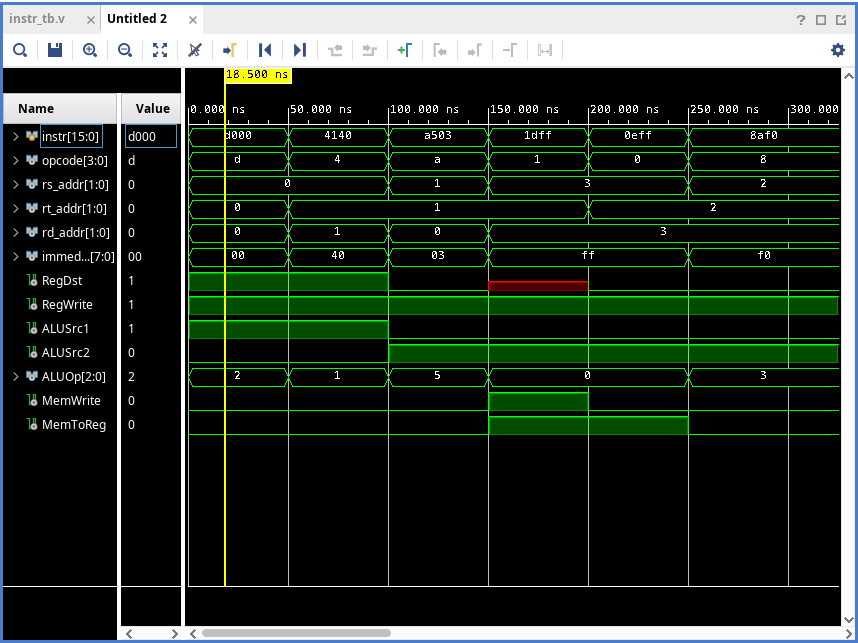
\includegraphics[width=\textwidth]{image}


\subsection*{Lab 7 toplevel.v}
\begin{lstlisting}
module pdatapath_top(
		input wire clk,				// General clock input
		input wire top_pb_clk,		// PBN1 clock input
        input wire rst_general,		// PBN0 clock reset for memory blocks
		output [7:0] led,			// add-on board led[5:0], + LD0, LD1
		output wire ovf_ctrl,    	// LD3 for overflow
		output [3:0] disp_en,		// 7-Segment display enable
		output [6:0] seg7_output	// 7-segment display output
    );

    // ALU inteface
    wire [7:0] alu_input1, alu_input2;
    wire [7:0] alu_output;
    wire [2:0] ALUOp;
    wire       alu_ovf;
    wire       take_branch;

    wire [15:0] instruction;
    //insturction fields
    wire [3:0] opcode;
    wire [1:0] rs_addr;
    wire [1:0] rt_addr;
    wire [1:0] rd_addr;
    wire [7:0] immediate;
    //control signals
    wire RegDst;
    wire RegWrite;
    wire ALUSrc1;
    wire ALUSrc2;
    wire MemWrite;
    wire MemToReg;

    wire [1:0] regfile_WriteAddress;//destination register address
    wire [8:0] regfile_WriteData;//result data
    wire [8:0] regfile_ReadData1;//source register1 data
    wire [8:0] regfile_ReadData2;//source register2 data

    wire [8:0] alu_result;
    wire [8:0] Data_Mem_Out;
    wire [7:0] zero_register;

    // PC and debouce clock
    wire [7:0] pc;
    wire pb_clk_debounced;

    assign zero_register = 8'b0;	//ZERO constant
    assign alu_result = {alu_ovf, alu_output};
	
    // Assign LEDs
    assign led = alu_output;
    assign ovf_ctrl = alu_ovf;

    // Debounce circuit
    debounce debounce_clk(
        .clk_in(clk),
        .rst_in(rst_general),
        .sig_in(top_pb_clk),
        .sig_debounced_out(pb_clk_debounced)
    );
	
    // 7-Segment display module
    Adaptor_display display(
	    .clk(clk), 					// system clock
	    .input_value(alu_output),	// 8-bit input [7:0] value to display
	    .disp_en(disp_en),			// output [3:0] 7 segment display enable
	    .seg7_output(seg7_output)	// output [6:0] 7 segment signals
    );

    //Instantiate Your PC Register here
    always@(posedge pb_clk_debounced or posedge rst_general)
    begin
        assign pc = rst_general ? 0 : pc + 1;
    end

    //Instantiate Your instruction Memory here
    instr_mem instruction_memory (
      .a(pc),      // input wire [7 : 0] a
      .spo(instruction)  // output wire [15 : 0] spo
    );

    instruction_decoder egiwu(
        .instr(instruction),
        .opcode(opcode),
        .rs_addr(rs_addr),
        .rt_addr(rt_addr),
        .rd_addr(rd_addr),
        .immediate(immediate),
        .RegDst(RegDst),
        .RegWrite(RegWrite),
        .ALUSrc1(ALUSrc1),
        .ALUSrc2(ALUSrc2),
        .ALUOp(ALUOp),
        .MemWrite(MemWrite),
        .MemToReg(MemToReg)
    );

    /* Instantiate the reg-file, MUXes, ALU that you have created here*/
    alu_regfile blast(
        .rst(rst_general),
        .clk(pb_clk_debounced),
        .rd0_addr(regfile_ReadAddress1),
        .rd1_addr(regfile_ReadAddress2),
        .wr_addr(regfile_WriteAddress),
        .wr_data(regfile_WriteData),
        .wr_en(RegWrite),
        .instr_i(alu_input2_instr_src),
        .alu_src2(ALUSrc1),
        .alu_src1(ALUSrc2),
        .alu_op(ALUOp),
        .result(alu_output),
        .input1(alu_input1),
        .input2(alu_input2),
        .ovf(alu_ovf),
        .take_branch(take_branch),
        .rd0_data(regfile_ReadData1),
        .rd1_data(regfile_ReadData2)
    );

   
    /* Instantiate the data memory that you have created here*/	
    data_memory dm (
      .a(alu_output),                // input wire [7 : 0] a
      .d(regfile_ReadData2),       // input wire [8 : 0] d
      .clk(clk),            // input wire clk
      .we(MemWrite),        // input wire we
      .spo(Data_Mem_Out)    // output wire [8 : 0] spo
    );
    /* Instantiate the VIO that you have created here, 
    make sure the number of probes and their width are correctly configured */

    assign regfile_WriteData = MemToReg ? Data_Mem_Out : alu_result;
	
    //Mux for RegDST
	
    assign regfile_WriteAddress = RegDst ? rd_addr : rt_addr;
    
    //Instantiate Your VIO core here


    //Didn't get to test a board so not sure if this is correct,
    //But it fully compiles when commented out.
    //Lab6 one seemed to work though (not posted because redundant).
    vio_0 vio(
       .clk(clk),
       .probe_in0(regfile_WriteData),
       .probe_in1(regfile_ReadData1),
       .probe_in2(regfile_ReadData2),
       .probe_in3(alu_input1),
       .probe_in4(alu_input2),
       .probe_in5(take_branch),
       .probe_in6(alu_ovf),
       .probe_in7(opcode),
       .probe_in8(alu_output),
       .probe_in9(Data_Mem_Out),
       .probe_out0(instruction)
    );

endmodule
\end{lstlisting}

\subsection*{Lab 7 Testing}

\begin{figure}
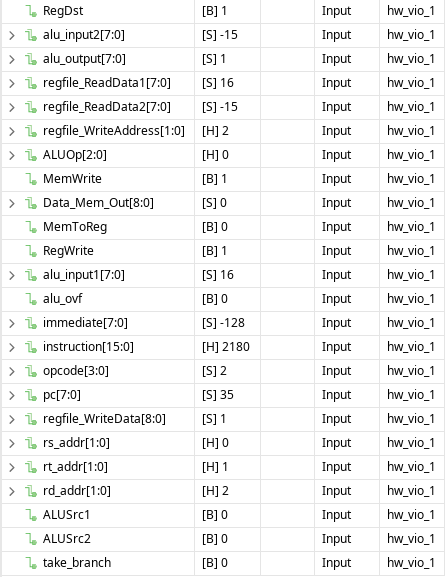
\includegraphics{image2}
\caption{Here we can see the correct number, 16-15 = 1, displayed in the alu\_out.}
\end{figure}


\end{document}
